\chapter{Android Aufnahmesystem}
\label{sec:androidaufnahmesystem}

Folgendes Kapitel behandelt das auf Google Android basierende Aufnahmesystem. Das Aufnahmesystem besteht aus zwei separaten Android Applikationen mit der Bezeichnung \textit{TourLive.apk} sowie \textit{TourLiveRecoveryService.apk}. Das Augenmerk folgender Unterkapitel liegt auf den Spezifikationen und der technischen Umsetzung des Aufnahmesystems und ist für Entwickler gedacht, die das Aufnahmesystem erweitern möchten.

\section{Software Analyse}
Dieses Kapitel beschreibt die Anforderungen an das Aufnahmesystem und gibt eine grobe  Übersicht über die vorhandene Funktionalität.

\subsection{Spezifikation}

Um die Anforderungen zu evaluieren wurde das bestehende Aufnahmesystem auf Basis von Nokia Symbian analysiert. Alle vorhandenen Funktionen wurden erfasst und gemeinsam mit dem Industriepartner um weitere ergänzt. 
Eine kurze Übersicht über die bereits bestehenden Funktionen und den neu erfassten Anforderungen liegt in tabellarischer Form vor.

\begin{longtable}{  p{3.5cm} | p{4.3cm} | p{4.3cm} }
    
    \textbf{Spezifikation} & \textbf{Altes System} & \textbf{Neues System} \\ [1ex] \hline \hline & &  \\ [-1.5ex]
    Positionsdaten übertragen & Geschwindigkeit, H\"{o}he, Richtung/Beschleunigung, Steigung, Longitude, Latitude & Geschwindigkeit, H\"{o}he, Richtung, Steigung, Longitude, Latitude \\ [1ex] \hline & &  \\ [-1.5ex]
    Etappendaten & Zeit, Höhe, Distanz, Durchschnittliche Geschwindigkeit, UTC Zeit, Datum & Zeit, Höhe, Distanz, Durchschnittliche Geschwindigkeit \\ [1ex] \hline & &  \\ [-1.5ex]
     Tour Total & Zeit Total, Zeit Tour, Distanz Total, Distanz Tour, Höhe Total, H\"{o}he Tour & - \\ [1ex] \hline & &  \\ [-1.5ex]
    Netzdaten übertragen & Zellen ID, Location Area, Signal, Akku, Netzwerk, Netzwerk ID & Zellen ID, Area, Signal, Netzwerk ID, Technologie, Datenrate\\ [1ex] \hline & &  \\ [-1.5ex]
    Bilder \"{u}bertragen & wird unterstützt & wird unterstützt \\ [1ex] \hline & &  \\ [-1.5ex]
    Videostream \"{u}bertragen & Einzelne Bilder wurden \"{u}bertragen und serverseitig zu einem Stream zusammengef\"{u}gt & Videosequenzen werden \"{u}bertragen und serverseitig zu einem Stream zusammengesetzt\\ [1ex] \hline & &  \\ [-1.5ex]
    Lokales Caching & nur Bilder wurden gecacht & S\"{a}mtliche aufgenommene Daten werden lokal gespeichert\\ [1ex] \hline & &  \\ [-1.5ex]
	Aufnahmegerät Systemstatus \"{u}bertragen & nur der Akkustand wurde an das Device Management Portal \"{u}bertragen & Detaillierte Statusinformation an das Device Management Portal\\ [1ex] \hline & &  \\ [-1.5ex]   
    Betriebsmodi & - & Managed - Einstellungen \"{u}ber das Portal / Unmanaged - Einstellungen am Ger\"{a}t\\ [1ex] \hline & &  \\ [-1.5ex]
	Auto-Start der App & - & App wird beim Ger\"{a}testart automatisch gestartet\\ [1ex] \hline & &  \\ [-1.5ex]
    Externe Ger\"{a}te & ODB (Onboard Diagnose Bus) und Pulsinfo Ger\"{a}te wurden angesteuert & -\\ [1ex] \hline & &  \\ [-1.5ex]
    Betriebssystem & Symbian App & Android App\\ [1ex] \hline & &  \\ [-1.5ex]
    Log & Position und Bilder gesendet & Daten, Bilder, Status und Einstellungen gesendet / Exceptions\\ [1ex] \hline & &  \\ [-1.5ex]
    Aufnahmestart Modi & Aufnahme hat automatisch bei App Start gestartet & Manuell, Zeitbasiert, Fernverwaltet oder bei Aktivierung einer externen Stromquelle\\ [1ex] \hline & &  \\ [-1.5ex]
   	Power Management & - & Bei niedrigem Akkustand wird ein Energiesparmodus aktiviert\\ [1ex] \hline & &  \\ [-1.5ex]
    Alarming Funktion & - & Treten Probleme auf, so wird darauf hingewiesen (z.B. keine GPS Daten w\"{a}hrend x Minuten)\\ [1ex] \hline & &  \\ [-1.5ex]
    Mehrsprachigkeit & - & Deutsch und Englisch, einfach erweiterbar\\ [1ex] \hline & &  \\ 
    [-1.5ex] Fehlerkorrektur der GPS Daten & - & Ausreisser bei den GPS Daten werden herausgefiltert\\ [1ex] \hline & &  \\ 
    [-1.5ex] Notfallwiederherstel- lung per SMS & wird unterstützt & wird unterstützt\\ [1ex]
    
\caption{Anforderungen Android Aufnahmesystem}
\end{longtable}

Eine detaillierte Beschreibung aller Anforderungen befindet sich im Anhang im Kapitel \ref{sec:anforderungenandroiddevmgmt}.

\section{Software Design}
Dieser Abschnitt dokumentiert das Software Design, verwendete Technologien und die Architektur des Aufnahmesystems.

\subsection{Verwendete Technologien}

\subsubsection{Android}
Eine Voraussetzung für das Aufnahmesystem ist, dass dieses in Form einer Android Applikation entwickelt wird. Die native Programmiersprache für Android Applikationen ist Android Java, ein der Java Standard Edition sehr ähnliches Java Derivat. Die Programmierung in Java bringt den Vorteil, dass die gesamte Android-\gls{api} benutzt werden kann. Da sämtliche Komponenten des TourLive Projektes in Java geschrieben sind,  kann teilweise auf Server- wie auch Clientseite auf dieselben Klassen-Bibliotheken zurückgegriffen werden, was mögliche Inkompatibilitäten vermindert. 

\paragraph{Android Version}
Eine Anwendung wird f"{u}r eine konkrete Android Version (Minimum Required SDK) entwickelt. Im Rahmen dieses Projektes wird als minimale SDK Version Android 4.0 (Versionsname: Ice Cream Sandwich\footnote{Android Ice Cream Sandwich, \url{http://www.android.com/about/ice-cream-sandwich/}, aufgerufen am 29.04.2013},  API-Level: 14) verwendet. Die Applikation sollte gemäss Android Richtlinien kompatibel mit allen darauffolgenden Android Versionen sein.

\subsection{Externe Libraries}
Um den geforderten Funktionsumfang umzusetzen, wird auf folgende zwei externe Bibliotheken zurückgegriffen.

\subsubsection{Spring for Android\footnote{Spring for Android, \url{http://www.springsource.org/spring-android}, aufgerufen am 29.04.2013} }
Ein Rest Client für Android von den Entwicklern des Java Spring Frameworks. Der Rest Client bietet die einfache Möglichkeit der Serialisierung / Deserialisierung von Java Objekten in JSON-Strings. 

Verwendete Version: spring-android-1.0.1

\subsubsection{ORMLite\footnote{ORMLite, \url{ormlite.com}, aufgerufen am 02.05.2013}} ORMLite ist eine OpenSource Java Library, welche das Object-Relational Mapping (ORM) übernimmt. ORMLite bietet eine speziell auf Android angepasste Distribution an. 

Verwendete Version: ORMLite-4.45

\subsection{Architektur des Aufnahmesystems}
Die Android Applikation zeichnet Daten für den TourLive Server sowie den Device Management Server auf. In der Abbildung \ref{fig:grobstrukturandroid}
 wird veranschaulicht, welche Daten an welchen Server übertragen werden.

\begin{figure}[H]
	\centering
	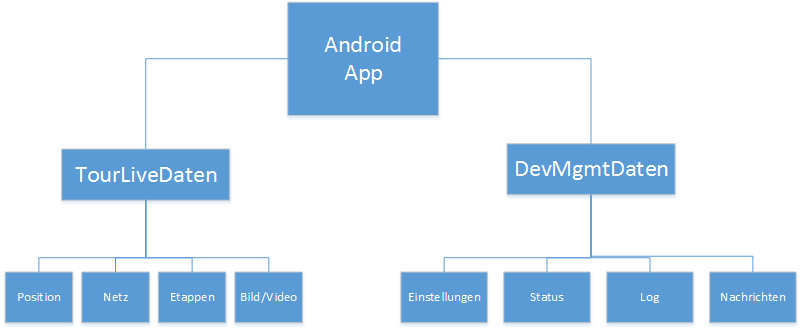
\includegraphics[width=120mm]{images/android/uebersicht.png}
	\caption{Grobstruktur der Android App}
	\label{fig:grobstrukturandroid} 
\end{figure}

\subsubsection{Schichtenmodell}
Die Android Applikation teilt sich in 3 Schichten auf.

\begin{figure}[H]
	\centering
	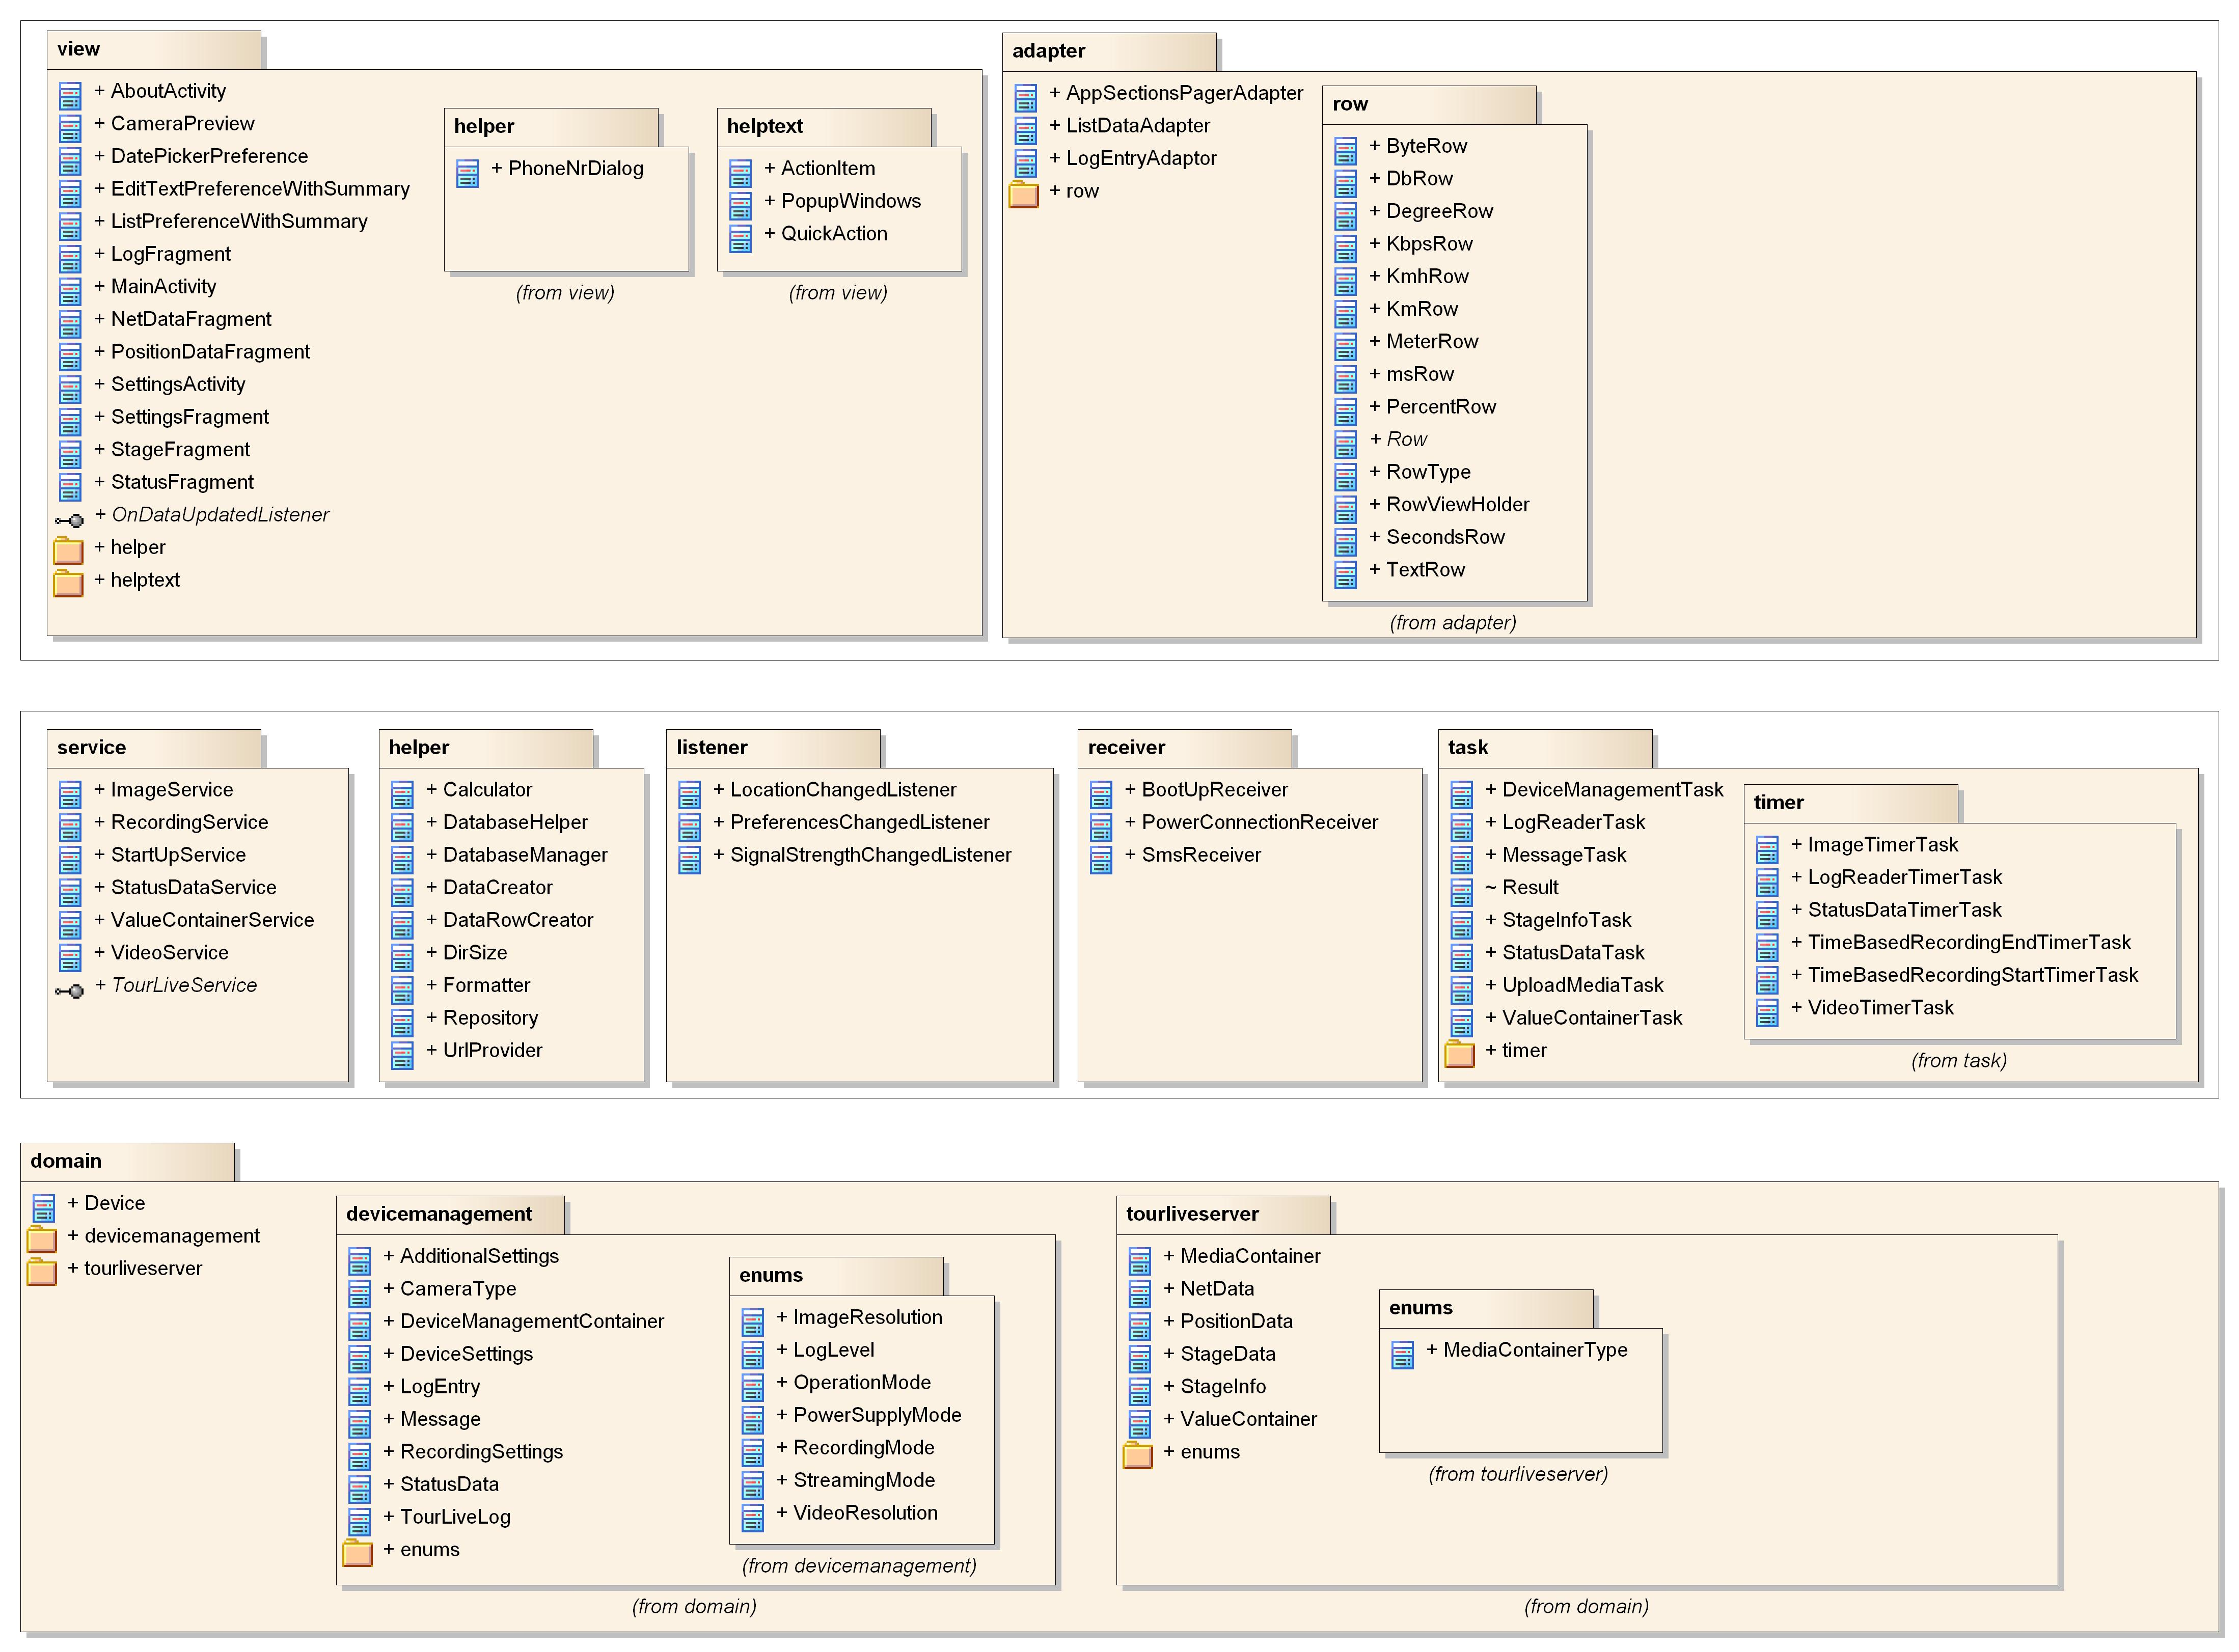
\includegraphics[width=150mm]{images/android/schichten.jpg}
	\caption{Packagediagramm des Aufnahmesystems}
\end{figure}

Die oberste Schicht stellt die Schnittstelle zum Benutzer dar. Die Klassen in dieser Schicht sind für die Darstellung zuständig. Die mittlere Schicht enthält die ganze Businesslogik. Dazu gehören Services, Timer, Listener, etc. Die unterste Schicht enthält die Domänenobjekte die die effektiven Daten (Positionsdaten, Konfigurationen, ...) enthalten. 

\subsubsection{Domain Model}
Das Domain Model des Aufnahmesystems setzt sich aus den Domain Models des TourLive Servers und des Device Management Servers zusammen. Im Aufnahmesystem kommen keine neuen Domänenobjekte hinzu.

\begin{figure}[H]
\centering
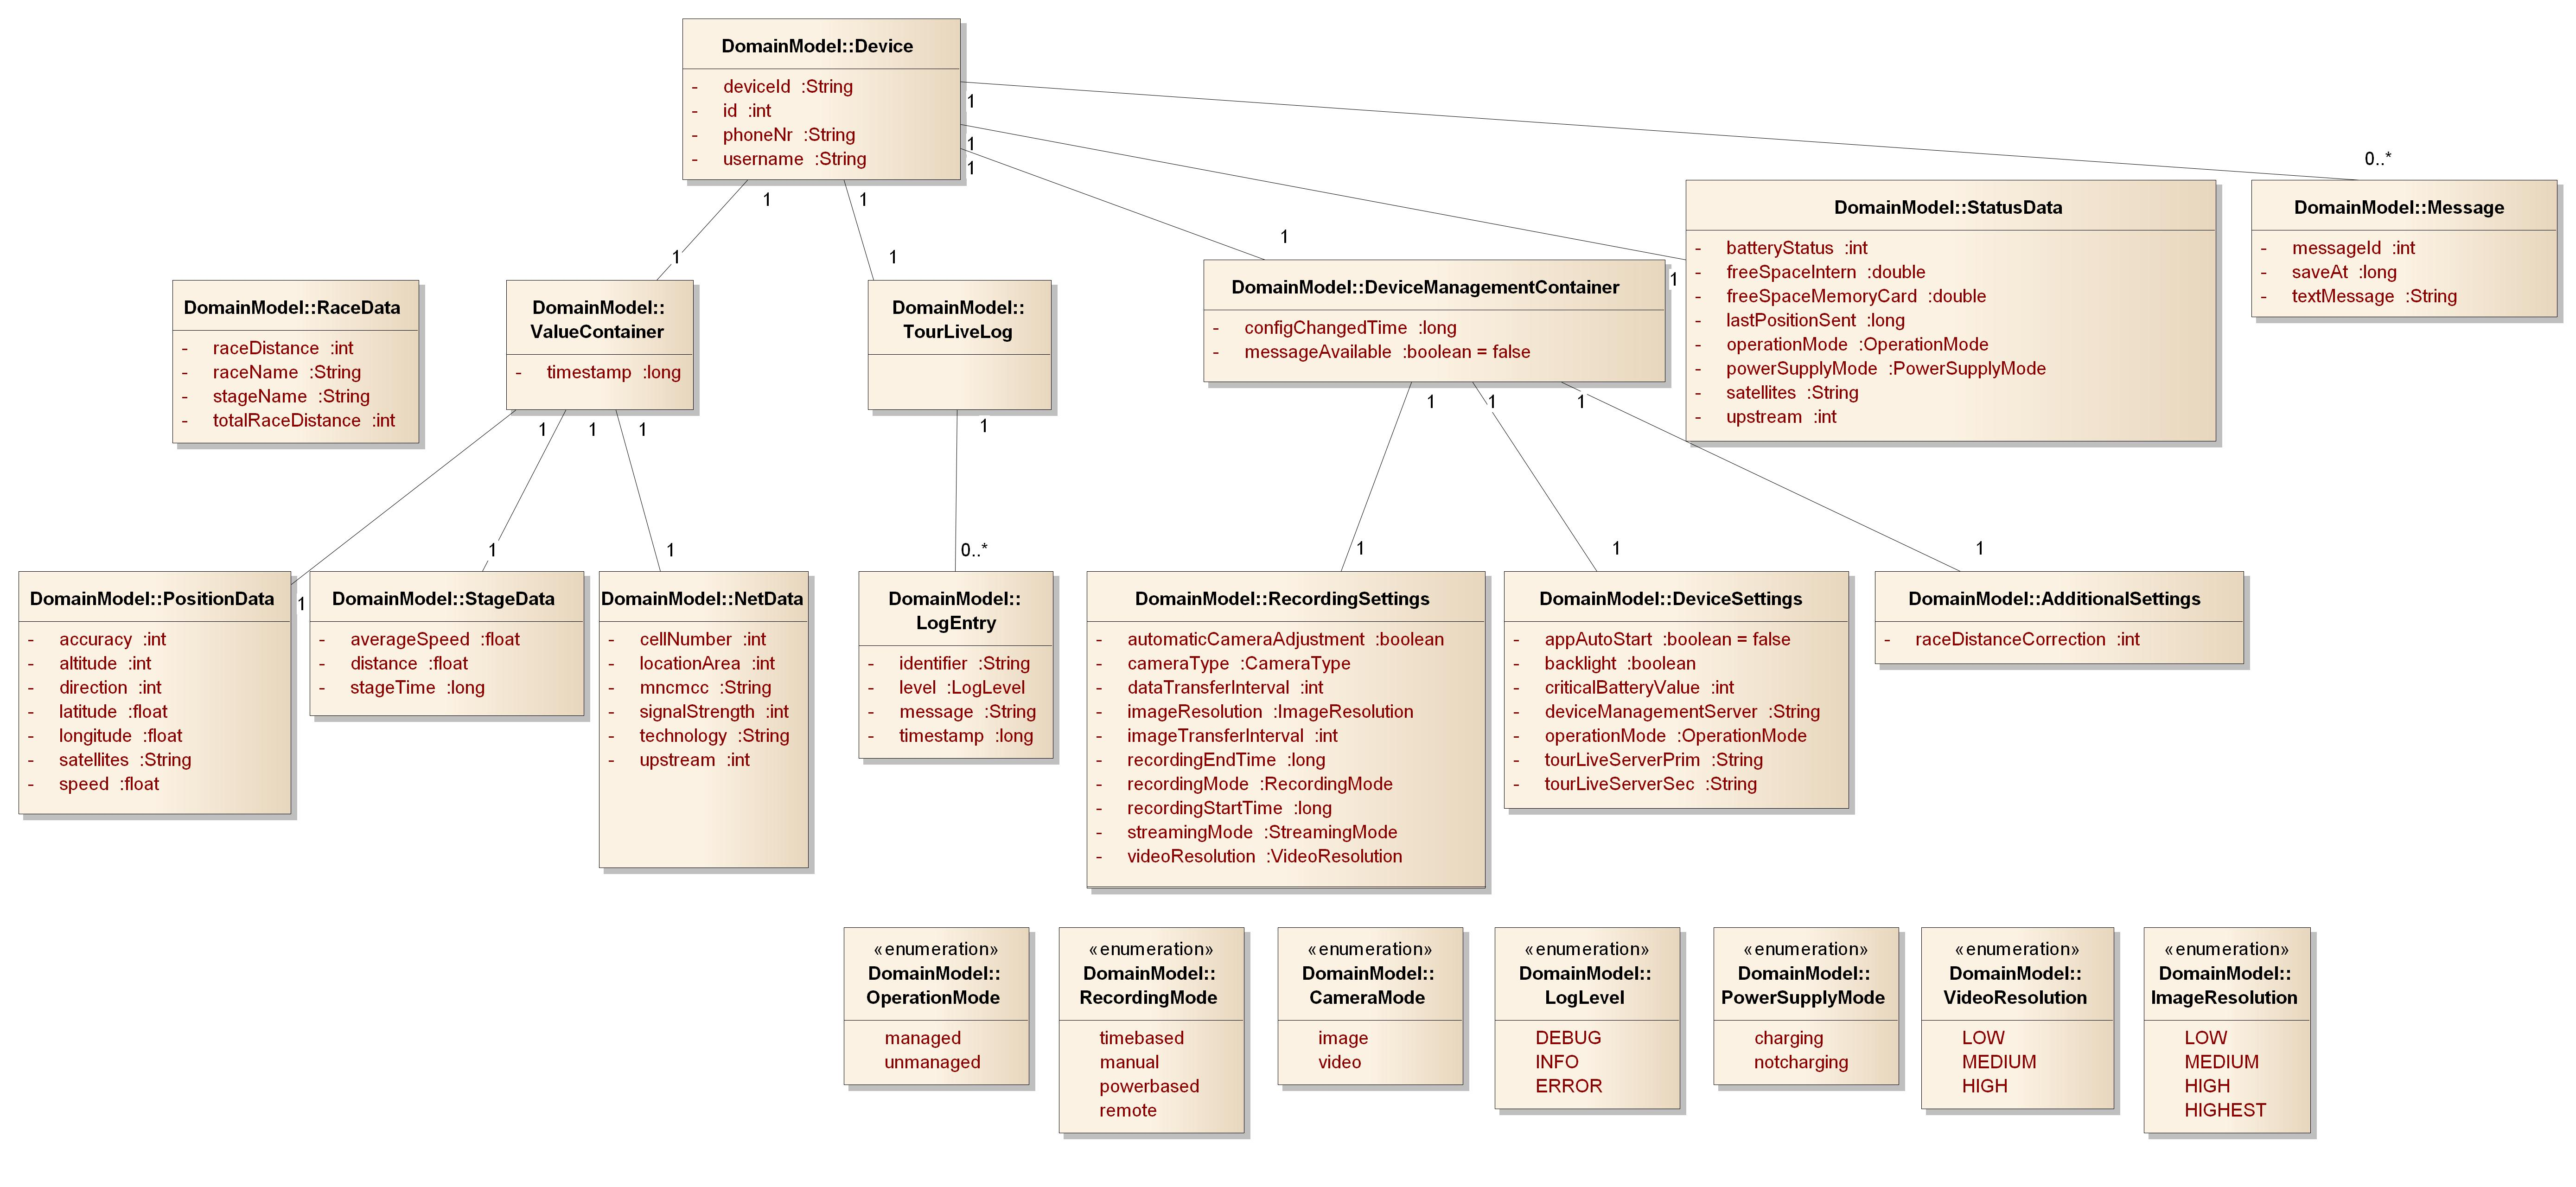
\includegraphics[width=130mm]{images/android/domainmodel.jpg}
\caption{Aufnahmesystem Domain Model}
\end{figure}

\subsubsection{Packagediagramm}
Die TourLive Applikation hat folgende Paketstruktur. Als Grundstruktur wurde analog zum TourLive Server und dem Device Management Server \textit{ch.hsr.ba.tourlive} verwendet. Die TourLive Applikation verwendet zusätzlich die Subkategorie \textit{.android} sowie folgende applikationsspezifische Struktur:

\begin{longtable}{p{5.0cm} | p{7.1cm}}
\textbf{Paket} & \textbf{Inhalt} \\
\hline \hline 
. & die initialisierende TourLiveApplication.java Klasse sowie Config.java \\ 
\hline 
.adapter & Daten-Adapter um Listen darzustellen \\ 
\hline 
.adapter.row & individuelle Listen Einträge \\ 
\hline 
.domain & projektübergreifende Domain Klassen \\ 
\hline 
.domain.devmgmtsrv & Device Management Server spezifische Domain Klassen \\ 
\hline 
.domain.devmgmtsrv.enums & Device Management Service spezifische Enums \\ 
\hline 
.domain.tourliveserver & TourLive Server spezifische Domain Klassen \\ 
\hline 
.domain.tourliveserver.enums & TourLive Server spezifische Enums \\  
\hline 
.helper & Hilfsklassen zur Berechnung von Werten \\ 
\hline 
.listener & System Event-Listener \\ 
\hline 
.receiver & Broadcast Receiver \\ 
\hline 
.service & sämtliche Services \\ 
\hline 
.task & sämtliche AsyncTasks \\ 
\hline 
.task.timer & sämtliche TimerTasks \\ 
\hline 
.view & Activities und Fragments \\ 
\hline 
.view.helper & individuelle Dialoge \\ 
\hline 
.view.helptext & die Hilfstext Klassen \\ 
\hline 
\end{longtable} 

\subsection{Architekturentscheide}

\subsubsection{Globaler Daten Provider - Repository.java}
Das Repository.java implementiert das Singleton-Pattern und fungiert als globaler Daten Provider. Damit werden lange Aufrufsketten verhindert. Das Repository bietet auf folgende Daten Zugriff:

\begin{itemize} [noitemsep,topsep=0pt]
	\item diverse Services
	\item das TourLiveLog
	\item Liste mit ValueContainers
	\item diverse globale Domänen Objekte
\end{itemize}

\subsubsection{Start der Applikation - TourLiveApplication.java}
Beim Start der TourLive Applikation müssen diverse Daten initialisiert werden. Um diese Initialisierung vor der ersten View durchzuführen wurde eine projektspezifische Klasse \textit{TourLiveApplication.java} geschrieben, die von der Android Klasse \textit{Application} ableitet. Eine von \textit{Application} abgeleitete Klasse darf nur einmalig vorkommen und wird als erste Klasse bei einem App-Start initialisiert.
\begin{quotation}
\textit{``Base class for those who need to maintain global application state''}.\footnote{Application class, \url{http://developer.android.com/reference/android/app/Application.html} besucht am: 10.04.2013}
\end{quotation}
Über die Klasse TourLiveApplication kann ausserdem auf den globalen Application-Context zugegriffen werden. Der zur Initialisierung diverser Objekte benötigt wird und wie folgt in den Android Developer Reference beschrieben ist.
\begin{quotation}
\textit{``Interface to global information about an application environment. This is an abstract class whose implementation is provided by the Android system. It allows access to application-specific resources and classes, as well as up-calls for application-level operations such as launching activities, broadcasting and receiving intents, etc.'' }\footnote{Context class, \url{http://developer.android.com/reference/android/content/Context.html} besucht am: 13.04.2013}
\end{quotation}

\subsubsection{Caching der Daten}
Um einen lokalen Cache zu realisieren wird der auf SQLite basierende OR-Mapper ORMLite verwendet. Der Cache verhindert Datenverlust bei Applikationsabstürzen. In der SQLite-Datenbank werden folgende Objekte gespeichert:

\begin{itemize} [noitemsep,topsep=0pt]
	\item Bildinformationen (Binärdatei liegt im Dateisystem)
	\item Videoinformationen (Binrädatei leigt im Dateisystem)
	\item Positions-, Etappen- \& Netzdaten (ValueContainer)
	\item Geräteinformationen (Device)
	\item Log-Einträge
\end{itemize}

Um Objekte und ihre Attribute zu persistieren, werden diese in den Modelklassen mit Java Annotationen markiert. 

\subsubsection{Factory Pattern - DataCreator.java}
Das erstellen der ValueContainer, DeviceManagementContainer und anderen Datenstrukturen unterliegt einem relativ komplexen Vorgang, da unzählige Werte aus den verschiedensten Android Listener,  Android Provider und Android Services zusammengezogen werden müssen. Das Factory Pattern schafft Abhilfe dies über ein einzelnes Objekt, den DataCreator, zu realisieren.

\subsubsection{Primärer / Sekundärer TourLive Server - URLProvider.java}
Eine Anforderung an das TourLive Aufnahmesystem ist die Implementation eines sekundären TourLive Servers, der bei Ausfall des primären Servers die Daten empfangen und verarbeiten kann. Dies wurde über die Klasse URLProvider.java realisiert. Schlägt die Verbindung zum aktuell ausgewählten Server, in der Regel ist dies der primäre Server, mehrmals fehl, stellt der URLProvider den Zweitserver zur Verfügung. Die Anzahl möglicher Fehlschläge vor einem Wechsel ist in der Config.java definiert. Sämtliche genutzten URLs werden über den URLProvider bezogen.

\subsubsection{Unveränderbare Applikationskonfiguration - Config.java}
In der \textit{Config.java} werden unveränderbare Applikationseinstellungen gespeichert. Diese sind direkt über \textit{public static final} Attribute aufrufbar. Die Config.java enthält folgende Konfigurationen:
\begin{itemize} [noitemsep,topsep=0pt]
	\item sämtliche API-URLs des TourLive Servers und des Device Management Servers
	\item Speicherort im Dateisystem der Bilddateien
	\item Speicherort im Dateisystem der Videodateien
	\item Intervall wie oft der Gerätezustand dem Device Management Server übertragen werden soll
	\item Angaben zur Genauigkeit die eine GPS Location haben muss, damit sie nicht verworfen wird
\end{itemize}

\section{Realisierung}
Das Kapitel Realisation gibt Hinweise zur Umsetzung des TourLive Aufnahmesystems. Es werden interne Abläufe und Funktionen erläutert und bietet eine kurze Einführung wie das Ausnahmesystem funktioniert. 

\subsection{Grafische Oberfläche}
\subsubsection{Einführung in die grafische Oberfläche von Android}

Die grafische Oberfläche einer Android Applikation besteht in erster Linie aus Activities. Gemäss Android Developer Reference wird eine Activity wie folgt definiert.

\begin{quotation}
\textit{``An activity is a single, focused thing that the user can do. Almost all activities interact with the user, so the Activity class takes care of creating a window for you in which you can place your UI.''} \footnote{Activity, \url{http://developer.android.com/reference/android/app/Activity.html}, besucht am: 25.03.2013}
\end{quotation}

Die TourLive Applikation wurde mit folgenden drei Activities realisiert.
\begin{itemize} [noitemsep,topsep=0pt]
	\item MainActivity.java
	\item SettingsActivity.java
	\item AboutActivity.java
\end{itemize}

Zu einer Activity gehört jeweils eine *.java Datei sowie eine *.xml Datei die das Layout definiert. Innerhalb einer Activity wird mit Fragments gearbeitet, welche wie folgt definiert sind:

\begin{quotation}
\textit{``A Fragment represents a behavior or a portion of user interface in an Activity.''} \footnote{Fragment, \url{http://developer.android.com/reference/android/app/Fragment.html}, besucht am: 25.03.2013}
\end{quotation}

Fragments werden für die verschiedenen Tabs innerhalb der MainActivity verwendet wie nachfolgende Screenshots zeigen.

\subsubsection{Konkrete Umsetzung der grafischen Oberfläche}
Die MainActivity, bestehend aus \textit{MainActivity.java} und \textit{main\_activity.xml}, ist die Hauptansicht der Applikation. Sie ist in drei Teile unterteilt, Header, Footer und Hauptbereich. Header und Footer sind in allen Tabs sichtbar.

\begin{figure}[H]
	\centering
	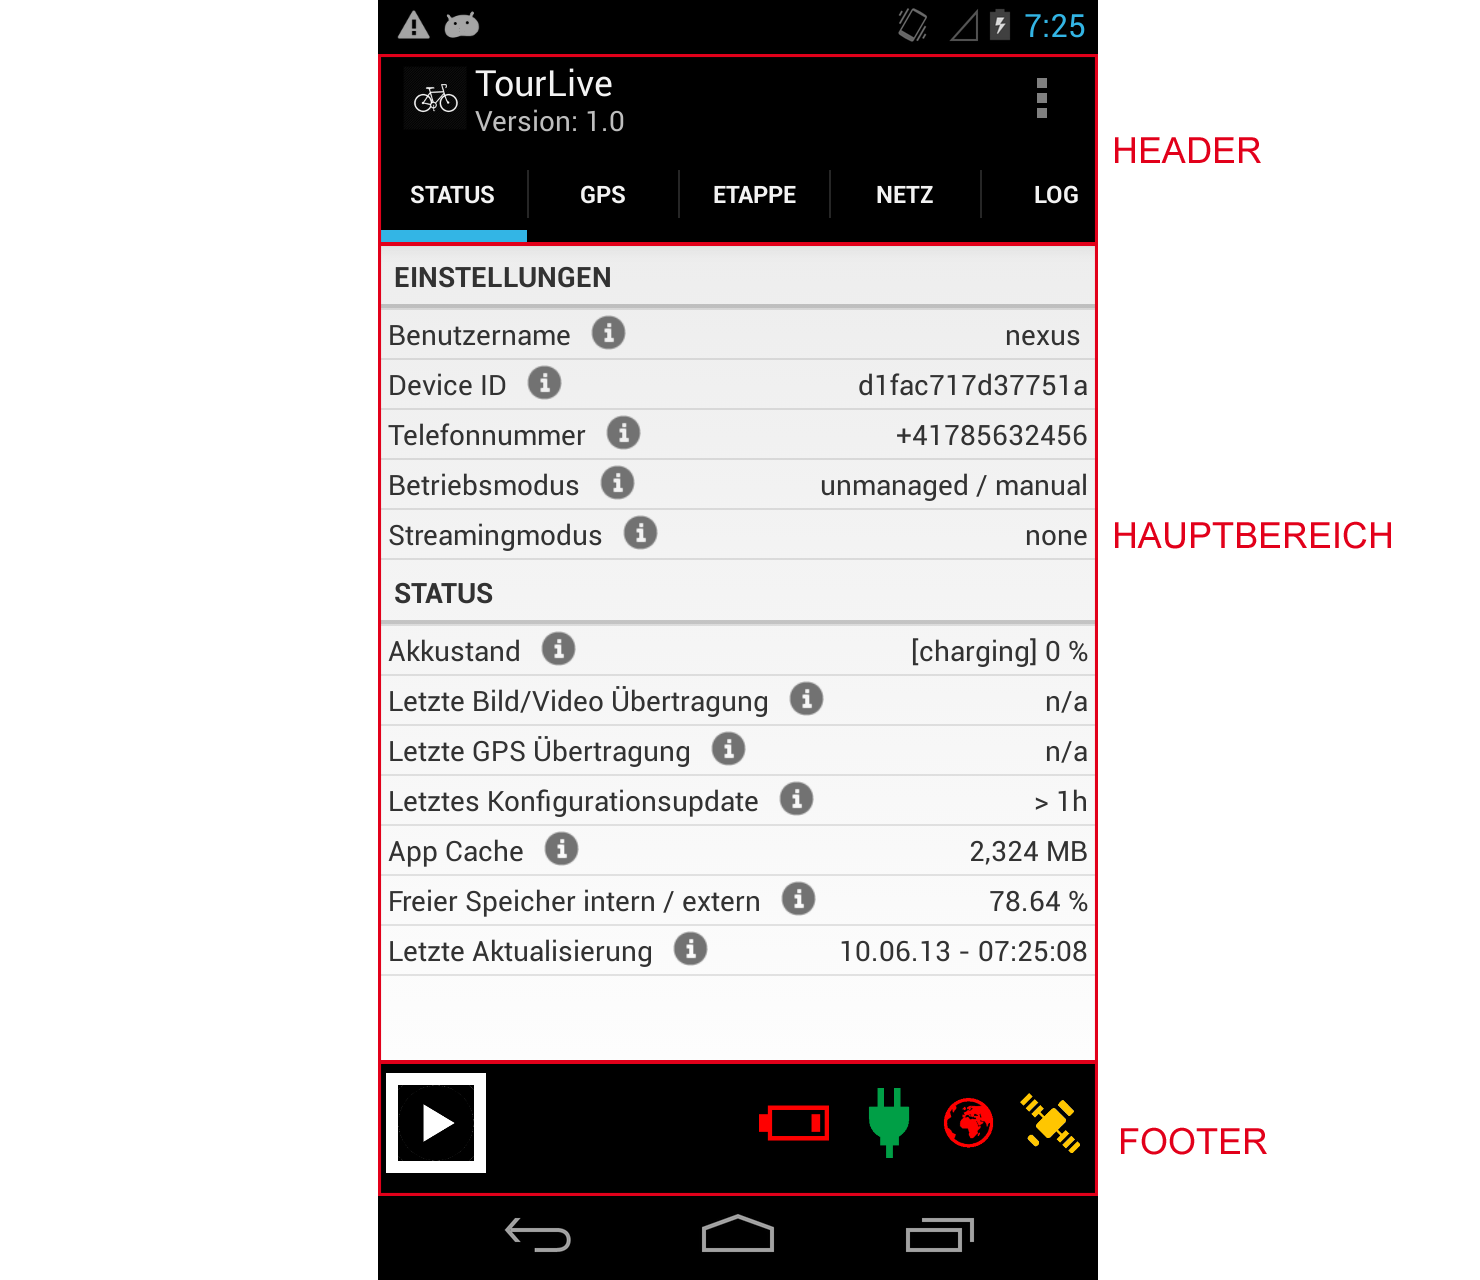
\includegraphics[width=120mm]{images/android/status.png}
	\caption{Aufnahmesystem MainActivity}
\end{figure}

\paragraph{Hauptbereich}
Der Inhalt des Hauptbereichs hängt vom selektierten Tab ab. Die einzelnen Ansichten Status, GPS, Etappe, Netz und Log wurden mit Fragments realisiert und basieren jeweils auf einer ListView.

\begin{quotation}
\textit{``ListView is a view group that displays a list of scrollable items. The list items are automatically inserted to the list using an Adapter that pulls content from a source such as an array or database query and converts each item result into a view that's placed into the list.''} \footnote{ListView, \url{http://developer.android.com/guide/topics/ui/layout/listview.html}, besucht am: 25.03.2013}
\end{quotation}

\paragraph{Header}
\begin{figure}[H]
	\centering
	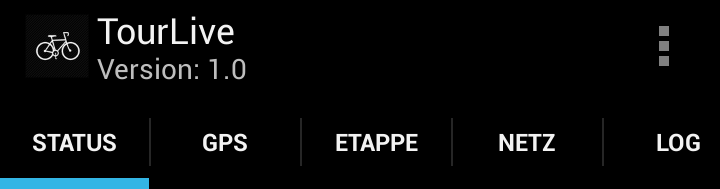
\includegraphics[width=60mm]{images/android/header.png}
	\caption{Aufnahmesystem Header}
\end{figure}
Der Header beinhaltet in der \textit{Action Bar} die aktuelle Versionsnummer, den Namen der Applikation sowie den Settings Button. Befindet sich die Applikation im Aufnahmemodus wird in roter Farbe der Text \textit{REC} eingeblendet. Unterhalb der \textit{Action Bar} befindet sich die \textit{Top Bar}, in der die verschiedenen Tabs angezeigt werden. Innerhalb des Content Bereiches kann mit einem Swipe zwischen den verschiedenen Views  hin und hergewechselt werden.

\paragraph{Settings Button}
Über den Settings Button wird folgendes Menü eingeblendet. Befindet sich die Applikation im Aufnahmemodus ist der Menüeintrag \textit{Einstellungen} deaktiviert. Die restlichen Aktionen sind trotzdem Verfügbar.

\begin{figure}[H]
	\centering
	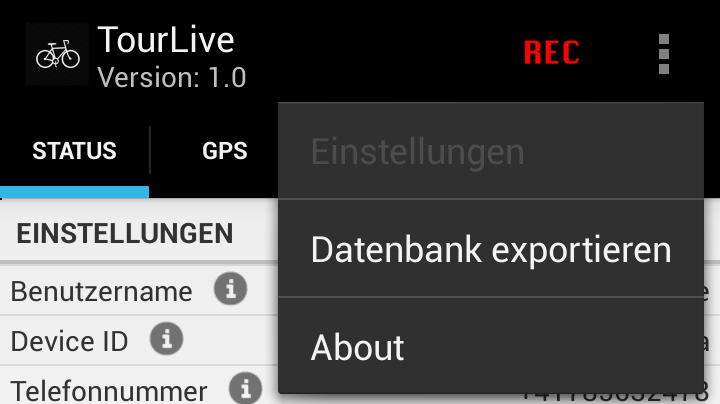
\includegraphics[width=60mm]{images/android/settingsclicked.png}
	\caption{Aufnahmesystem Settings Button Clicked}
\end{figure}



\paragraph{Footer}
\begin{figure}[H]
	\centering
	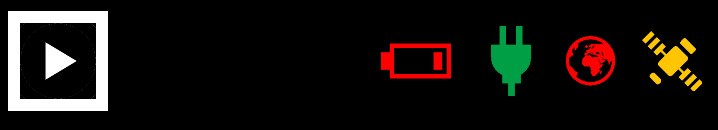
\includegraphics[width=60mm]{images/android/footer.png}
	\caption{Aufnahmesystem Footer}
\end{figure}
Der Footer zeigt den Status der App. Die Symbole werden je nach Gesundheitszustand der Applikation rot, gelb oder grün dargestellt. Welche Farbe welchem Gesundheitszustand entspricht, ist in den Anforderungen im Kapitel \ref{par:alarming} beschrieben.\\

Mit dem Recording Button links kann die Aufnahme gestartet und gestoppt werden. Der Button ist nur aktiviert, wenn der Aufnahmemodus auf manuell gesetzt ist.

\paragraph{Einstellungen}
\begin{figure}[H]
	\centering
	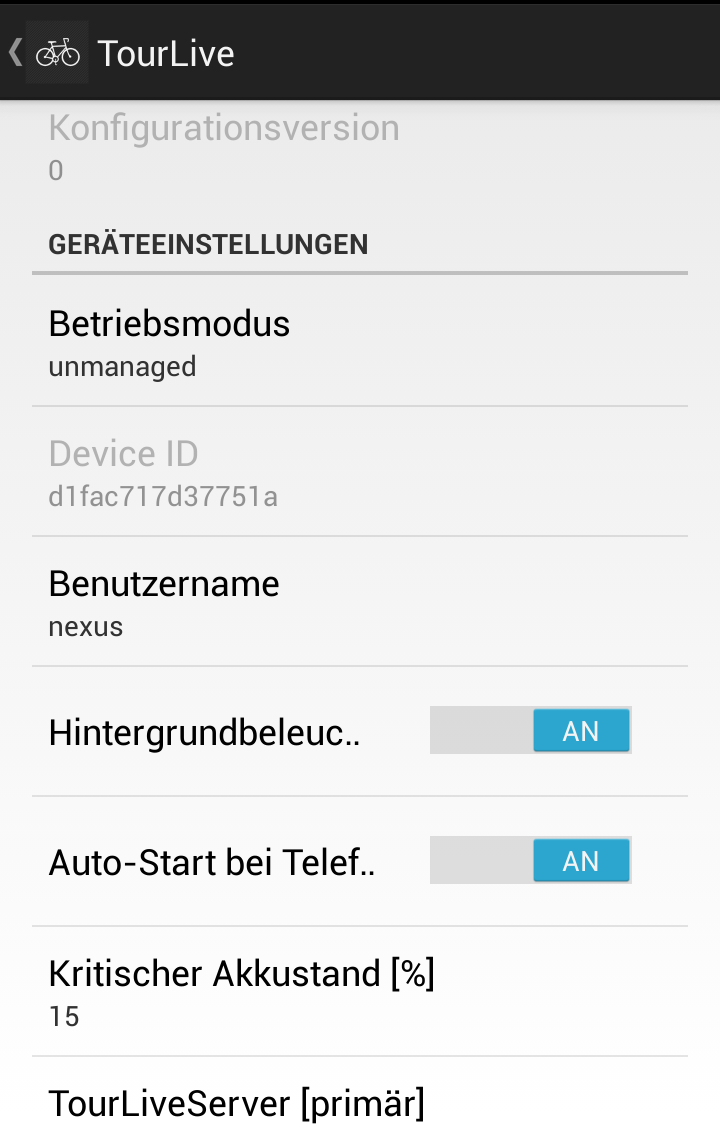
\includegraphics[width=60mm]{images/android/settings.png}
	\caption{Aufnahmesystem Einstellungen}
\end{figure}

Der oben abgebildete Screenshot zeigt einen Ausschnitt der Aufnahmesystemeinstellungen. Sämtliche Einstellungen können auch am Device Management Server verwaltet werden und werden regelmässig synchronisiert. Folgende Einstellungen sind möglich:

\begin{itemize}
	\item Konfigurationsversion (read-only)
	\item Betriebsmodus (managed / unmanaged)
	\item Device ID (read-only)
	\item Benutername (String)
	\item Hintergrundbeleichtung (on / off)
	\item Auto-Start bei Gerätestart (on / off)
	\item Kritischer Akku-Stand (0 - 100 \%)
	\item TourLive Server primär (String)
	\item TourLive Server sekundär (String)
	\item Device Management Server primär (String)
	\item Aufnamemodus (manuell, strombasiert, ferngesteuert, zeitbasiert)
	\item Startzeit (DateTimePicker - nur bei Aufnahmemodus zeitbasiert)
	\item Endzeit (DateTimePicker - nur bei Aufnahmemodus zeitbasiert)
	\item Datenübertragunsintervall (Integer)
	\item Kamera automatisch ausrichten (on / off)
	\item Kamera (front / back)
	\item Streamingmodus (Bilder / Videos / Nichts)
	\item Bildauflösung (320x240, 640x480, 1280x960, 1600x1200)
	\item Bildübertragunsintervall (Integer)
	\item Videoauflösung (176x144, 720x480, 1280x720)
	\item Renndistanzkorrektur (Integer)
\end{itemize}
Es ist ausserdem möglich sämtliche lokal gespeicherten Etappen und Positionsdaten zu löschen, sämtliche Bilder und Videodaten zu löschen und die Telefonnummer beim Wechsel der SIM-Karte anzupassen.

\subsection{Berechtigungen}
Das Starten einer Android Applikation erfordert je nach Funktionalität der Applikation bestimmte Systemberechtigungen, die bei der Installation \textit{Akzeptiert} werden müssen.
\begin{figure}[H]
	\centering
	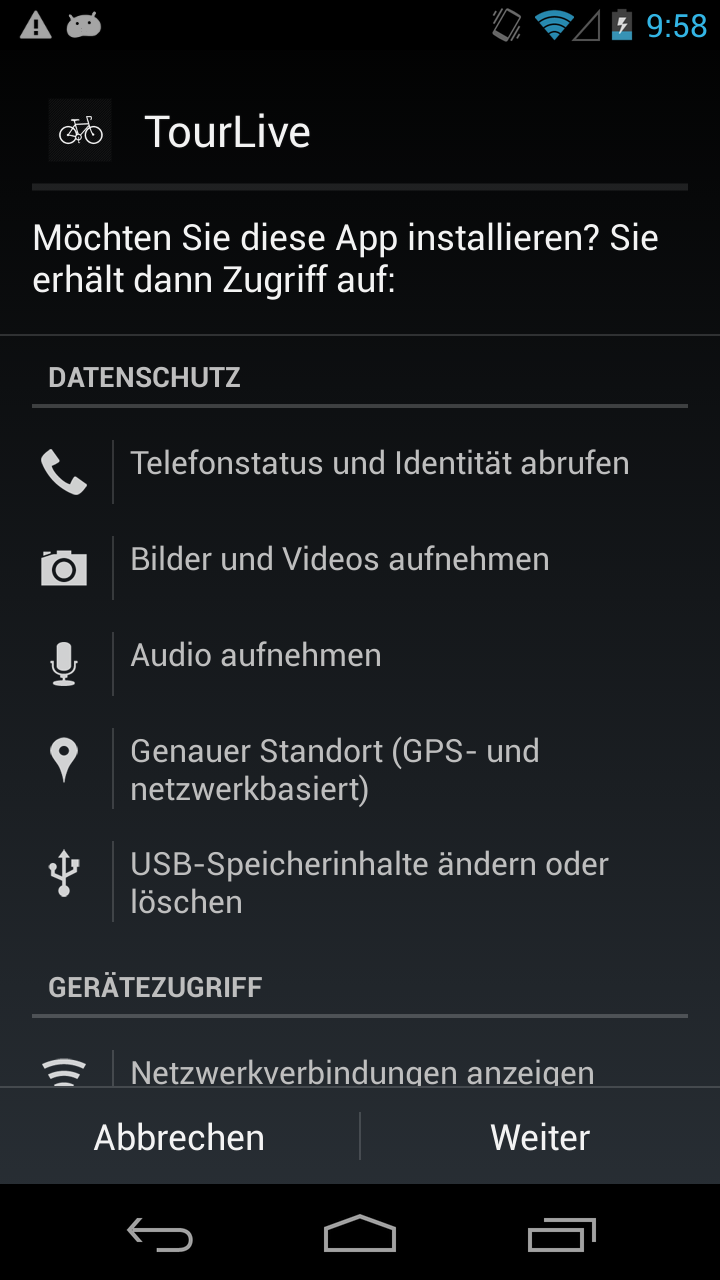
\includegraphics[width=60mm]{images/android/berechtigungen.png}
	\caption{Aufnahmesystem Berechtigungen}
\end{figure}
\subsubsection{Datenschutz}

\begin{itemize} [noitemsep,topsep=0pt]
	\item \textbf{Telefonstatus und Identität abrufen:} Berechtigt das auslesen der Telefonnummer
	\item \textbf{Bilder und Videos aufnehmen:} Berechtigt die Aufnahme von Bildens und Videos
	\item \textbf{Audio aufnehmen:} Berechtigt die Aufnahme von Audio
	\item \textbf{Genauer Standort:} Berechtigt die Nutzung des GPS Providers
	\item \textbf{USB Speicherinhalte ändern und löschen:} Berechtigt den Zugriff auf das Dateisystem (Bilder und Videos)
\end{itemize}

\subsubsection{Gerätezugriff}
\begin{itemize} [noitemsep,topsep=0pt]
	\item \textbf{Netzwerkverbindungen:} Berechtigt zur Nutzung des mobilen Netzwerks
	\item \textbf{Beim Start ausführen:} Berechtigt die Nutzung des Auto-Starts
	\item \textbf{Zugriff auf geschützten Speicher testen:} Berechtigt den Zugriff auf das Dateisystem (SQLite)
\end{itemize}

\subsection{I18N}
Die Applikation ist in deutscher sowie englischer Sprache verfügbar. Weitere Sprachen lassen sich einfach durch erstellen  und übersetzen der Ordnerstruktur TourLive/res/values-SPRACHE hinzufügen.

\subsection{Services, Tasks \& TimerTasks}
Die TourLive Applikation arbeitet mit mehreren Services. Diese implementieren in der Regel das eigens für diese Applikation entworfene Interface \textit{TourLiveService.java}. Die Services werden in der Regel in Verbindung mit einem \textit{Timer} genutzt der wiederum einen \textit{TimerTask} voraussetzt.

\begin{quotation}
\textit{``Each timer has one thread on which tasks are executed sequentially. When this thread is busy running a task, runnable tasks may be subject to delays.''} \footnote{Timer, \url{http://developer.android.com/reference/java/util/Timer.html}, besucht am: 11.04.2013}
\end{quotation}

\begin{quotation}
\textit{``The TimerTask class represents a task to run at a specified time. The task may be run once or repeatedly.''} \footnote{TimerTask, \url{http://developer.android.com/reference/java/util/TimerTask.html}, besucht am: 11.04.2013}
\end{quotation}

Folgende Services, Timer und TimerTask werden in der TourLive Applikation verwendet.
\subsubsection{RecordingService} 
\textit{RecordingService.java} ist verantwortlich für die Aufnahme von Live Informationen. Wird entweder manuell über den Start-Button, via Device Management Server über den Fernstart, strom- oder zeitbasiert gestartet. Direkt mit dem RecordingService verknüpft sind folgende Services: ValueContainerService, ImageService und der VideoService.
\subsubsection{ValueContainerService} 
\textit{ValueContainerService.java} ist für die Übertragung von Positionsdaten (ValueContainer) verantwortlich. Der ValueContainerService registriert einen LocationListener der GPS-Updates meldet und diese dann mit Hilfe des DataCreators in ValueContainer-Objekt erstellt und per ValueContainerTask an den TourLive Server überträgt.
\subsubsection{ImageService} 
\textit{ImageService.java} ist für die Übertragung von Bilddaten verantwortlich. Der ImageService terminiert mit der Unterstützung eines Timers den TimerTask \textit{ImageTimerTask.java} der in regelmässigem Intervall ein Einzelbild aufnimmt und dieses per \textit{UploadMediaTask.java} an den TourLive Server sendet. 
\subsubsection{VideoService} 
\textit{VideoService.java} ist für die  Übertragung von Videodaten verantwortlich. Analog zum ImageService nutzt der VideoService den \textit{VideoTimerTask.java} zur Aufnahme von Videosequenzen und den gemeinsamen UploadMediaTask.java zur Übertragung der Videosequenzen an den TourLive Server.
\subsubsection{StartUpService} 
\textit{StartUpService.java} ist für den Auto-Start der Applikation nach dem Gerätestart verantwortlich, sofern dieser in den Einstellungen aktiviert ist.
\subsubsection{StatusDataService} 
\textit{StatusDataService.java} ist für die  Übertragung des Gerätezustandes verantwortlich. Mit Hilfe eines Timers und des \textit{StatusDataTimerTask.java} wird in regelmässigem Intervall der Gerätezustand an den Device Management Server übertragen.

\subsection{Kommunikation mit den Servern}
Für die Übertragung der Daten an die beiden Server wurden AsyncTasks verwendet. Diese ermöglichen eine einfache Anwendung von Threads und sind in der Android Developer Reference wie folgt definiert: 

\begin{quotation}
\textit{``AsyncTask enables proper and easy use of the UI thread. This class allows to perform background operations and publish results on the UI thread without having to manipulate threads and/or handlers. An asynchronous task is defined by a computation that runs on a background thread and whose result is published on the UI thread. An asynchronous task is defined by 3 generic types, called Params, Progress and Result, and 4 steps, called onPreExecute, doInBackground, onProgressUpdate and onPostExecute.''} \footnote{AsyncTask, \url{http://developer.android.com/reference/android/os/AsyncTask.html}, besucht am: 13.04.2013}
\end{quotation}

Es folgt eine kurze Auflistung der implementieren AsyncTasks.
\begin{itemize} [noitemsep,topsep=0pt]
	\item \textit{DeviceManagementTask.java} überträgt die Einstellungen an den Device Management Server und registriert das Gerät beim Applikationsstart.
	\item \textit{LogReaderTask.java} aktualisiert die LogView alle 5 Sekunden.
	\item \textit{MessageTask.java} bezieht Nachrichten vom Device Management Server, sofern welche vorhanden sind
	\item \textit{StageInfoTask.java} bezieht Renn- und Etappeninformationen vom TourLive Server
	\item \textit{StatusDataTask.java} sendet den Gerätezustand an den Device Management Server und empfängt allfällige Konfigurationsänderungen vom Device Management Server. 
	\item \textit{UploadMediaTask.java} sendet Bild- und Videodaten an den TourLive Server
	\item \textit{ValueContainerTask.java} sendet Positionsdaten an den TourLive Server
\end{itemize}

\subsection{Listener \& BroadcastReceiver}
Listener und BroadcastReceiver empfangen System- und andere Events. 
\begin{itemize} [noitemsep,topsep=0pt]
	\item \textit{LocationChangedListener.java} meldet Positionsupdates.
	\item \textit{PreferenceChangedListener.java} meldet Einstellungsänderungen.
	\item \textit{SignalStrengthListener.java} meldet Signalstärkenänderungen.
	\item \textit{BootUpReceiver.java} meldet einen Gerätestart.
	\item \textit{PowerConnectionReceiver.java} meldet Änderungen in der Stromversorgung.
\end{itemize}

\subsection{Aufnahme von Bildern und Videosequenzen}
Die Aufnahme von Bild- und Videosequenzen kann über die Android API grundsätzlich ziemlich komfortabel realisiert werden. Vorausgesetzt wird lediglich eine View (Bereich auf dem Bildschirm) die als Kamera Vorschau genutzt werden kann. 

\begin{quotation}
\textit{``Sets the Surface to be used for live preview. Either a surface or surface texture is necessary for preview, and preview is necessary to take pictures.''} \footnote{AsyncTask, \url{http://developer.android.com/reference/android/hardware/Camera.html\#setPreviewDisplay\%28android.view.SurfaceHolder\%29}, besucht am: 17.04.2013}
\end{quotation}

Eine View wiederum muss mit einer Activity verknüpft werden und eine Activity wiederum kennt verschiedene Status (\textit{active}, \textit{paused}, \textit{stopped}, \textit{destroyed}). Welche Activity sich in welchem Status befindet wird vom Android Betriebssystem verwaltet. Grundsätzlich kann aber davon ausgegangen werden, dass eine Activity sich nicht mehr im Status \textit{active} befindet, wenn die Applikation sich im Hintergrund befindet oder der Bildschirm sich abdunkelt. Befindet sich eine Activity nicht mehr im Status \textit{active} kommt es vor, dass der Garbage Collector View-Objekte aufräumt die beim reaktivieren der Activity neu initialisiert werden.

Mit diesem Verhalten der Android API gibt es zwei Konflikte mit den Anforderungen an die TourLive Applikation. 

Das erste Problem mit der geforderten View die als Vorschau benötigt wird,  kann mit einer 1x1 Pixel grossen View die ``unsichtbaren'' in einer Ecke angezeigt wird, gelöst werden. 

Das zweite, etwas grössere Problem besteht darin, dass Bilder und Videosequenzen auch aufgenommen werden sollen, wenn die Applikation im Hintergrund oder mit abgedunkelten Bildschirm läuft. Da in diesen beiden Fällen die Möglichkeit besteht, dass die MainActivity in einen anderen Status als \textit{active} wechselt, kann es vorkommen, dass die View für die Kamera Vorschau vom Garbage Collector aufgeräumt wird. In diesem Fall muss die MainActivity neu gestartet und die View für die Kamera Vorschau neu initialisiert werden. 

Da die Android Kamera Design Prinzipien nicht für einen solchen Verwendungszweck ausgelegt ist (Aufnahme ohne Vorschau, Aufnahme bei abgedunkeltem Bildschirm / Applikation im Hintergrund) kann es während dem Betrieb zu unvorhergesehenen Problemen (Exceptions) kommen.

\subsection{Datenbank}
Für das lokale Caching werden Daten mittels ORMLite in die Datenbank geschrieben. Eine Klasse wird mittels Annotation als Datenbankklasse definiert.

\begin{lstlisting}[language=Java, caption=ORMLite Annotations]
@DatabaseTable
public class Device {
	@DatabaseField(generatedId = true)
	private int id;
	@DatabaseField
	private String deviceId;
	@DatabaseField
	private String username;
	@DatabaseField
	private String phoneNr;
}
\end{lstlisting}

\begin{itemize}
\item \textbf{\textit{@DatabaseTable}:} mit dieser Annotation wird angegeben, dass die annotierte Klasse  eine gemappte Datenbank Klasse ist.
\item \textbf{\textit{@DatabaseField}:} das folgende Attribut ist eine Spalte in der Datenbank. Mittels generatedID = true wird für das Attribut eine eindeutige ID generiert.
\end{itemize}


Die Klasse \textit{DatabaseHelper.java} verwaltet die Zugriffe auf die Datenbank. Beim ersten Start der App werden die Tabellen generiert. Werden später neue Attribute hinzugefügt, so muss die Datenbankversion erhöht und in der \textit{onUpgrade} - Methode ein Update-Script zur Verfügung gestellt werden.\\

Der \textit{DatenbankManager.java}, eine Singleton Klasse, ermöglicht den Zugriff über den \textit{DatabaseHelper.java} auf die Datenbank. Im \textit{DatenbankManager.java} sind sämtliche \textit{\gls{CRUD}}-Operationen enthalten.

\subsection{Systemsequenzdiagramme}
Dieses Kapitel beschreibt die Abläufe innerhalb der Applikation in Form von Systemsequenzdiagrammen. Sie geben eine grobe Übersicht wie die bisher erwähnten Klassen zusammenarbeiten.

\subsubsection{Applikation im Ruhezustand}
Diagramm \ref{fig:permanenttasks} beschreibt die Applikation im Ruhezustand. In regelmässigem Intervall (wird in der \textit{Config.java} definiert.) wird der Gesundheitszustand des Gerätes an den Device Management Server übertragen. Der Device Management Server antwortet mit der gespeicherten Gerätekonfiguration des Gerätes sowie einem Message-Flag, dass kennzeichnet wenn eine Nachricht für das Gerät vorhanden ist. 

Sind keine Renn- und Etappeninformationen vorhanden oder sind diese veraltet, werden diese nach Beendigung des ersten Requests beim TourLive Server abgerufen.

Wurde zudem das Message-Flag gesetzt, wird in einem weiteren Request die Nachricht abgerufen. 

 
\begin{figure}[H]
	\centering
	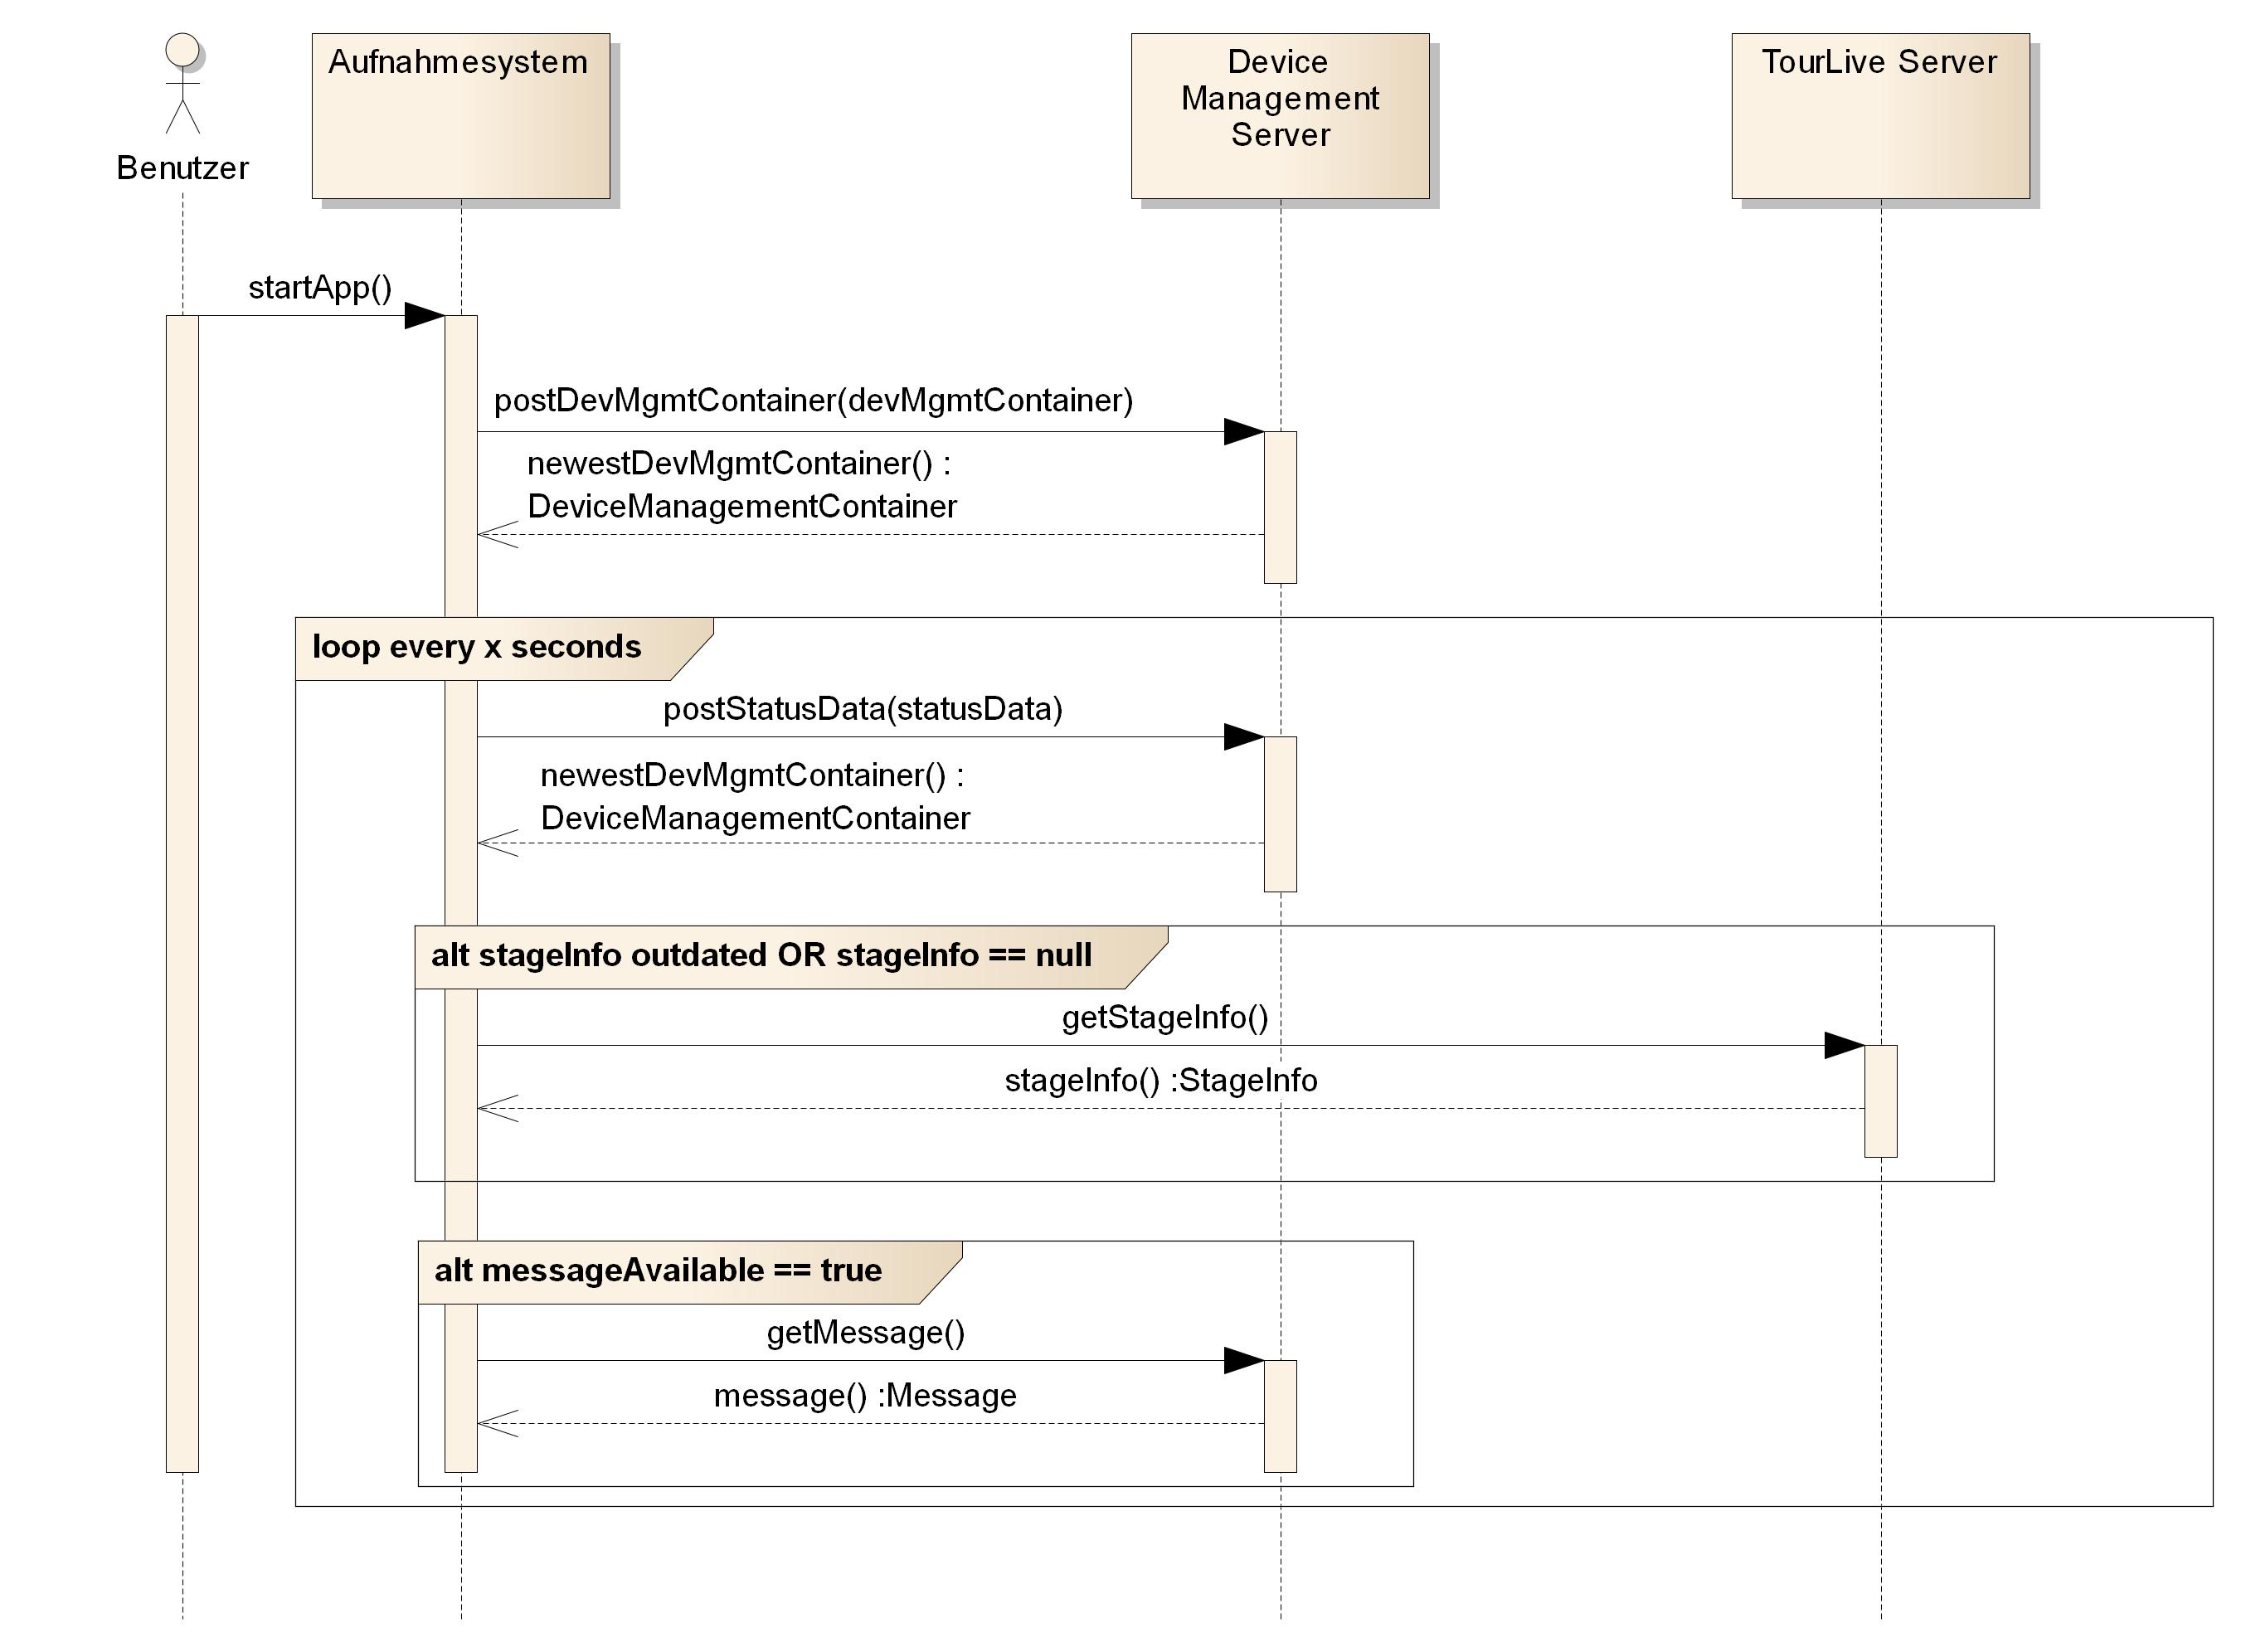
\includegraphics[width=150mm]{images/android/permanent_taskes.jpg}
	\label{fig:permanenttasks}
	\caption{Aufnahmesystem permanente Tasks}
\end{figure}

\subsubsection{Applikation im Aufnahmemodus}
Diagramm \ref{fig:recording} zeigt die Abläufe beim Starten des Aufnahmemodus (\textit{RecordingService.java}). Die Operation \textit{startRecording()} entspricht dem \textit{RecordingService.java}. Der Start des RecordingServices beinhaltet auf jeden Fall den Start des  \textit{ValueContainerService.java}. Je nach Konfiguration wird zudem der \textit{VideoService.java}, der \textit{ImageService.java} oder keiner der beiden gestartet.

\begin{figure}[H]
	\centering
	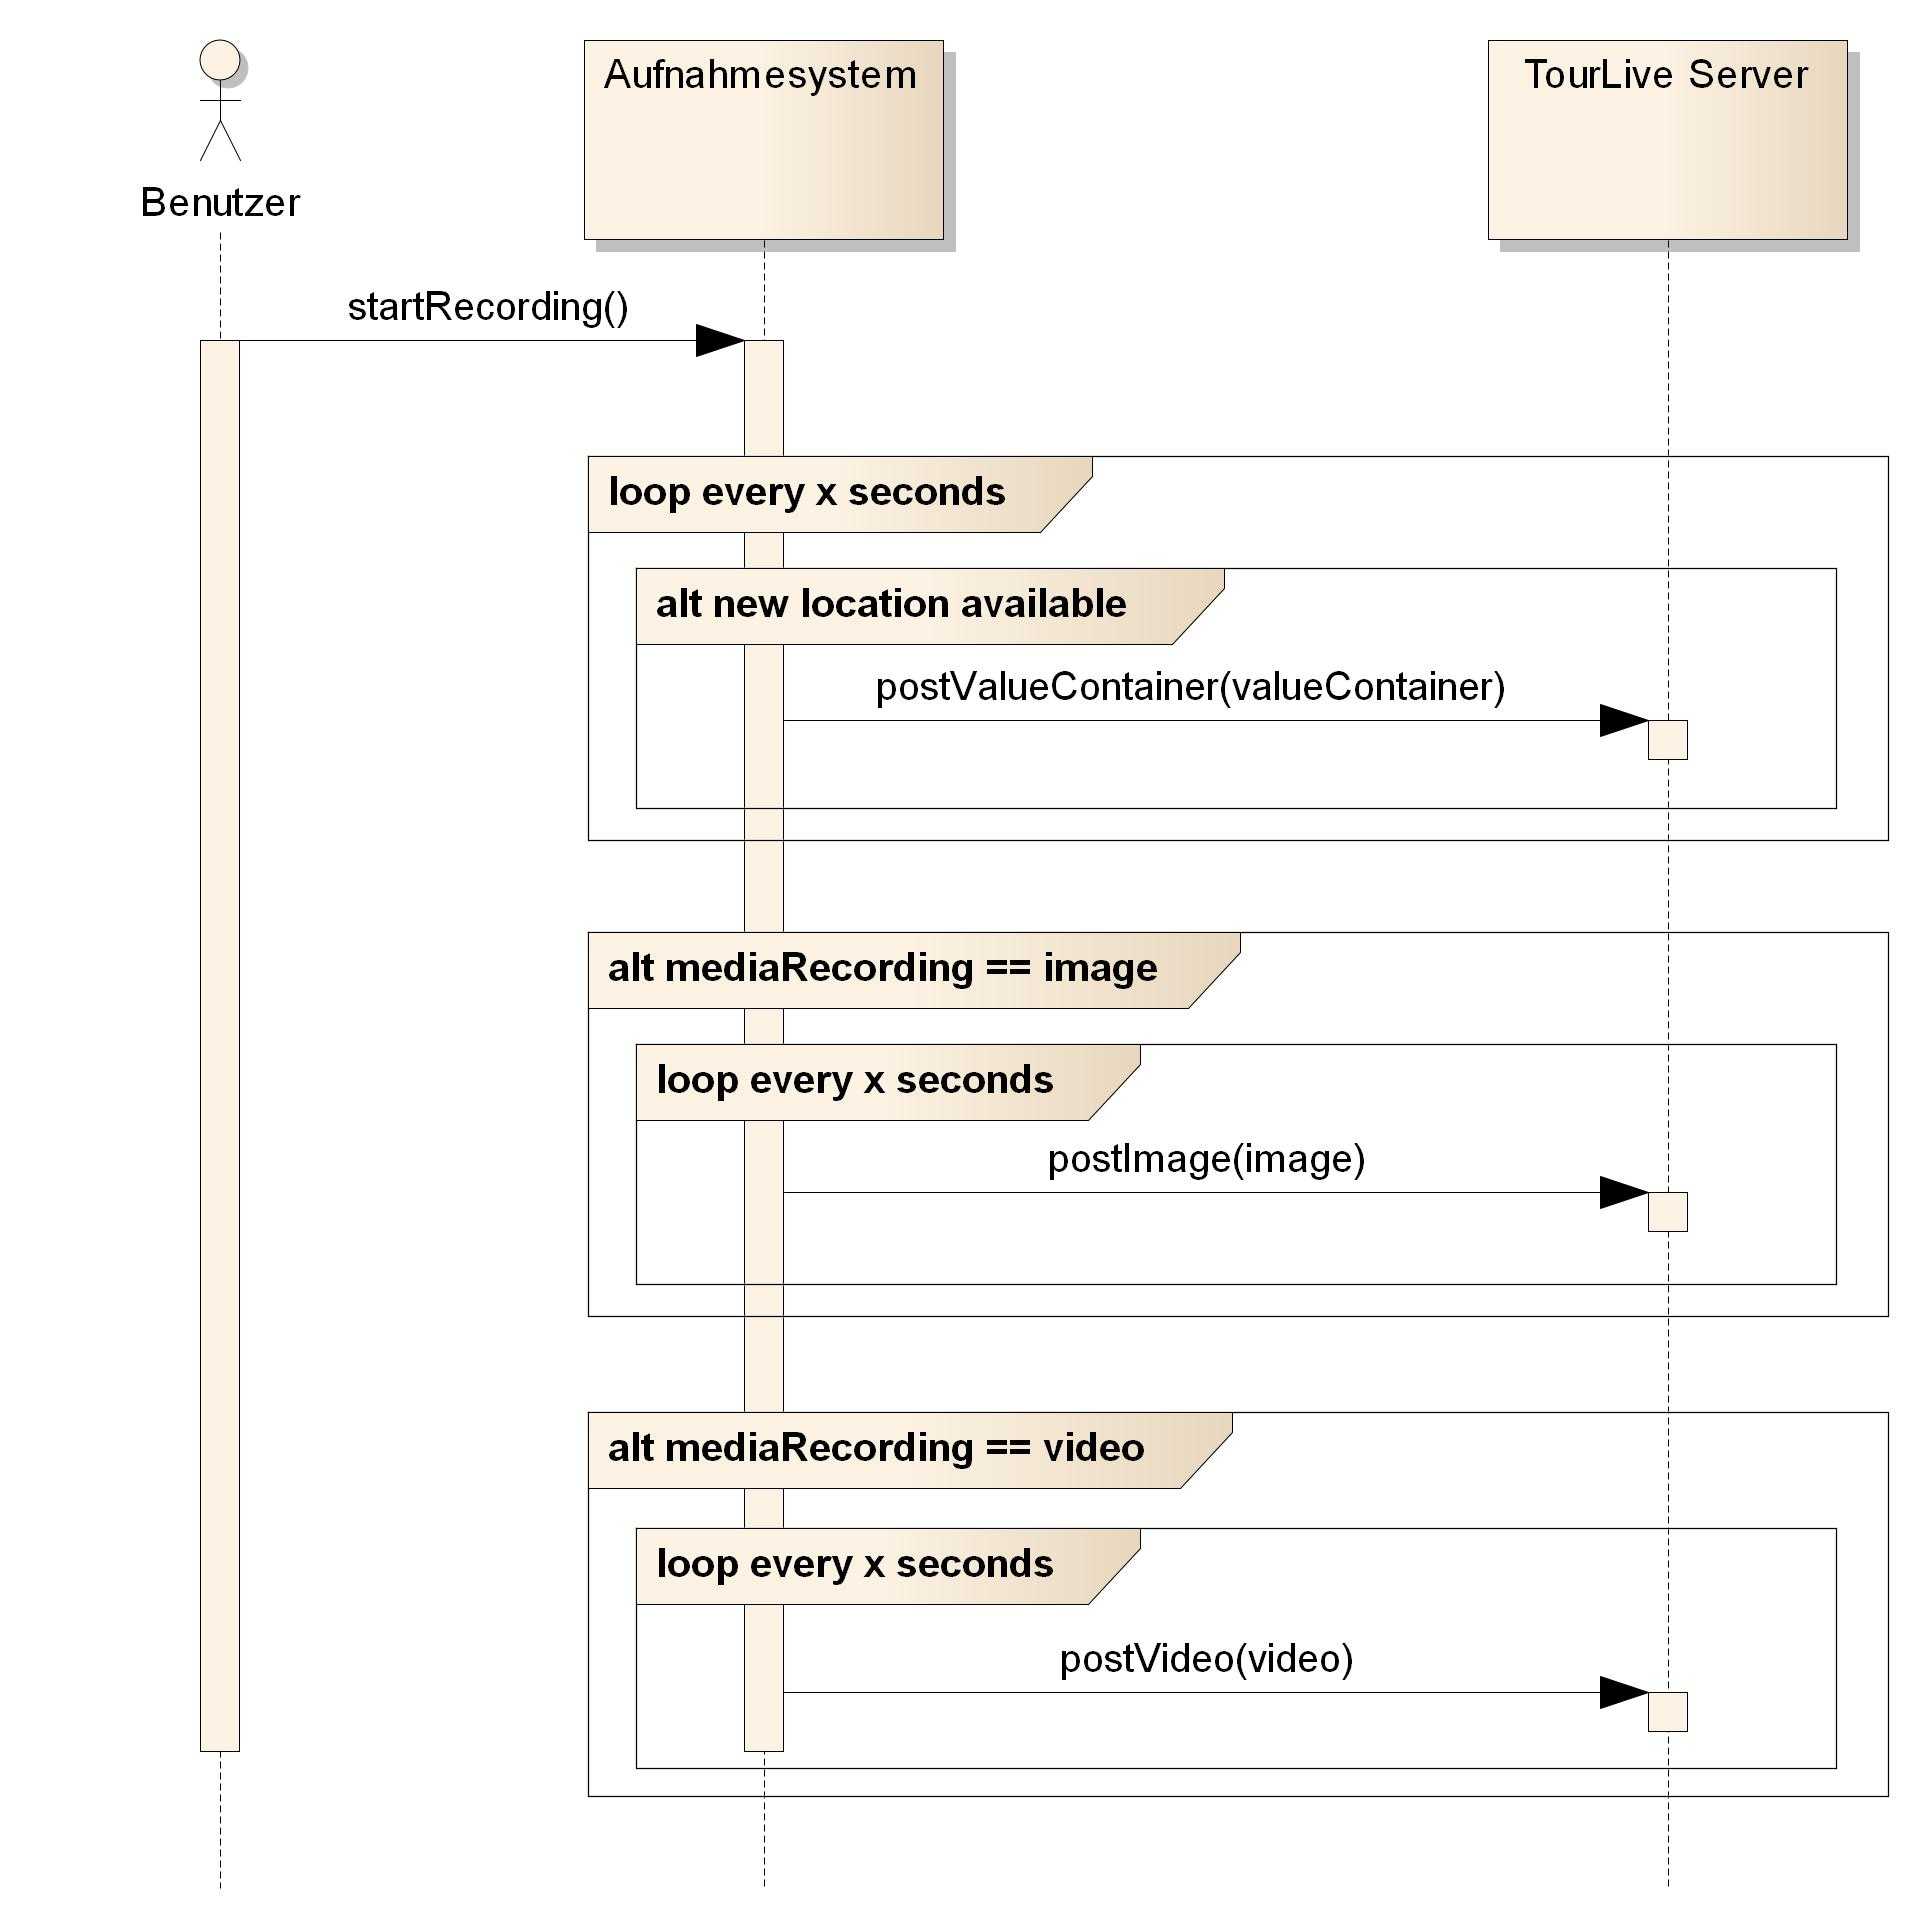
\includegraphics[width=150mm]{images/android/recording.jpg}
	\label{fig:recording}
	\caption{Aufnahmesystem Aufnahme}
\end{figure}

\subsection{Algorithmen}
Das Aufnahmesystem enthält einige Algorithmen zur Berechnung von Distanzen, Steigungen und Zeit. Diese werden im folgenden Abschnitt kurz beschrieben. Damit eine Berechnung durchgeführt werden kann wird ein \textit{StageInfo}-Objekt vorausgesetzt, das beschreibt, in welchem Rennen beziehungsweise in welcher Etappe sich das Aufnahmegerät aktuell befindet.
\\

\subsubsection{Berechnung der Renndauer}
Die Renndauer ist in der TourLive Applikation im Tab Etappe (eng. Stage) zu finden und beschreibt die Renndauer seit dem offiziellen Etappenstart gemäss \textit{StageInfo}. Die Berechnung der Renndauer erfolgt durch eine einfache Subtraktion.


\begin{algorithm}[H]
\begin{algorithmic}[1]
\vspace{5pt}
\If {$StageInfo \neq null$}
     \State \Return $now$ - $StageInfo.StageStartTime$;
\Else
     \State \Return $0$;
\EndIf
\end{algorithmic}
\caption{Berechnung der Renndauer}
\end{algorithm}


Die Renndauer wird bei der Erstellung eines \textit{ValueContainers} im assoziierten \textit{StageData} im Attribut \textit{stageTime} gespeichert.

\subsubsection{Berechnung der überwundenen Höhenmeter}
Die überwundenen Höhenmeter repräsentieren das Total der positiv überwundenen Höhenmeter während einer Etappe. Der Wert wird in der TourLive Applikation im Tab Etappe (eng. Stage) angezeigt. Die Berechnung erfolgt nach folgendem Algorithmus.

\begin{algorithm}[H]
\begin{algorithmic}[1]
\vspace{5pt}
\State $Altitude \gets 0$;
\State $CurrentAltitude \gets null$;
\State $NextAltitude \gets null$;
\ForAll{$ValueContainers$ since $StageInfo.StageStartTime$}
\If {$NextAltitude \neq null$}
\State $CurrentAltitude \gets ValueContainer.Altitude$;
\If {$CurrentAltitude \leq NextAltitude$}
     \State $Altitude\gets Altitude + (NextAltitude - CurrentAltitude)$
\EndIf
\Else
\State $NextAltitude \gets ValueContainer.Altitude$;
\EndIf
\EndFor
\end{algorithmic}
\caption{Berechnung der überwundenen Höhenmeter}
\end{algorithm}


Die überwundenen Höhenmeter werden bei der Erstellung eines \textit{ValueContainers} im assoziierten \textit{StageData} im Attribut \textit{stageUpAltitude} gespeichert.

\subsubsection{Berechnung der Steigung}
Die Angabe zur Steigung beziehen sich auf die letzten 100m Horizontaldistanz. Die Steigung wird im Tab Etappe (eng. Stage) angezeigt und bei der Erstellung eines \textit{ValueContainers} im assoziierten \textit{StageData} als Attribut \textit{incline} gespeichert. Die Berechnung erfolgt nach folgendem Algorithmus.


\begin{algorithm}[H]
\begin{algorithmic}[1]
\vspace{5pt}
\State $Altitude \gets 0$;
\State $Distance \gets 0$;
\State $LastAltitude \gets null$;
\State $LastDistance \gets null$;
\ForAll{$ValueContainers.Reverse$}
\If {$valueContainer$ is in $currentStage$}
\State $CurrAltitude \gets ValueContainer.Altitude$;
\State $CurrDistance \gets ValueContainer.Distance$;
\If {$LastAltitude \neq null$ \textbf{and} $LastDistance \neq null$ }
\State $Altitude \gets Altitude + (LastAltitude - CurrAltitude)$;
\State $Distance \gets Distance + (LastDistance - CurrDistance)$;
\EndIf
\State $LastAltitude \gets CurrAltitude$;
\State $LastDistance \gets CurrDistance$;
\If {$Distance \geq 100$}
\State BREAK;
\EndIf
\Else
\State BREAK;
\EndIf
\EndFor
\State $Incline \gets altitude/distance$;
\State \Return $arctan(incline.toDegrees)$;
\end{algorithmic}
\caption{Berechnung der Steigung}
\end{algorithm}

\subsubsection{Allgemeine Algorithmen zur Vermeidung von Berechnungsfehlern}
Die Erstellung eines ValueContainers erfolgt sobald das Aufnahmegerät eine neue Position meldet. Es kann vorkommen, dass die GPS-API von Android fehlerhafte Positionsdaten liefert. Aus diesem Grund werden erstellte ValueContainer auf ihre Datenkonsistenz überprüft und gegebenenfalls wieder verworfen. Der ValueContainer wird nach folgenden Kriterien überprüft:
\begin{itemize} [noitemsep,topsep=0pt]
\item longitude != 0
\item latitude != 0
\item accuracy < 100m
\item returned location from GPS\_PROVIDER != null
\end{itemize}

\subsection{TourLive Recovery Service}
Die Notfallwiederherstellung wie sie in den Anforderungen ans Aufnahmesystem formuliert ist, wurde aus Gründen der Zuverlässigkeit und Stabilität als separate Android Applikation (\textit{TourLiveRecoveryService.apk}) realisiert. Der TourLiveRecoveryService startet beim Gerätestart automatisch und besteht aus zwei Komponenten. Der SmsReceiver scannt einkommende SMS nach dem Stichwort \textit{RESTART} und sendet, falls dieses Stichwort gefunden wurde, eine Nachricht (Intent) an die TourLive Applikation um diese nach einem Absturz erneut zu starten. 
